\documentclass[a4j]{jarticle}
    \usepackage[dvipdfmx]{graphicx}
    \usepackage[ top=25truemm,bottom=37truemm,left=25truemm,right=25truemm]
    {geometry}
    \usepackage{ascmac}
    \usepackage{array}
    \usepackage{amsmath}
    \usepackage{here}
    \usepackage{url}
    \usepackage{listings, jlisting}
    \usepackage{cases}
    \usepackage[subrefformat=parens]{subcaption}
    \renewcommand{\lstlistingname}{リスト}
\lstset{language=c,
  basicstyle=\ttfamily\scriptsize,
  commentstyle=\textit,
  classoffset=1,
  keywordstyle=\bfseries,
  frame=tRBl,
  framesep=5pt,
  showstringspaces=false,
  numbers=left,
  stepnumber=1,
  numberstyle=\tiny,
  tabsize=4
}

\makeatletter
\def\@thesis{シミュレーション レポート}
\def\id#1{\def\@id{#1}}
\def\department#1{\def\@department{#1}}

\def\@maketitle{
\begin{center}
{\huge \@thesis \par} %修士論文と記載される部分
\vspace{10mm}
{\LARGE\bf \@title \par}% 論文のタイトル部分
\vspace{10mm}
{\Large \@date\par}	% 提出年月日部分
\vspace{20mm}
{\Large \@department \par}	% 所属部分
{\Large 学籍番号 \@id \par}	% 学籍番号部分
\vspace{10mm}
{\Large 氏名 \@author}% 氏名 
\end{center}
\par\vskip 1.5em
}

\title{第11回~第15回}
\date{提出日 2021年2月5日}
\department{組番号 408}
\id{17406}
\author{金澤雄大}

    \begin{document}
    \maketitle
    \thispagestyle{empty}
    \clearpage
    \addtocounter{page}{-1}
    \section{目的}
    シミュレーションの授業で学習したアルゴリズムを実装し,数値計算を行うことを目的とする.

    \section{実験環境}
      実験環境を表\ref{env}に示す. gccはWindows上のWSL(Windows Subsystem for Linux)で動作するものを用いる.
      \begin{table}[H]
        \caption{実験環境}
      \label{env}
      \begin{center}
          \begin{tabular}{c|l}\hline
            CPU & AMD Ryzen 5 3600 6-Core Processor \\ 
            メモリ & 16.0GB DDR4 \\
            OS & Microsoft Windows 10 Home \\
            gcc & (Ubuntu 9.3.0-17ubuntu1~20.04) 9.3.0 \\
            Make & GNU Make 4.2.1 \\ \hline
          \end{tabular}
      \end{center}
      \end{table}

      \section{課題11}
      本章では課題11のプログラム,実行結果,手計算の3つについて述べる.
      \subsection{プログラム}
      リスト\ref{kadai11}に課題11のコードを示す.
      \begin{lstlisting}[basicstyle=\ttfamily\footnotesize, frame=single,label=kadai11,caption=課題11のコード]
#include<stdio.h>
#define N 4

double x[N]={0,0,0,0};

double A[N][N]={{1,2,1,5},
                {8,1,3,1},
                {1,7,1,1},
                {1,1,6,1}};
double b[N]={20.5,14.5,18.5,9.0};

void disp(double A[N][N],double b[N]){
    int i,j;
    printf("--------------------\n");
    for(i=0;i<N;i++){
        for(j=0;j<N;j++){
            printf("%.2lf ",A[i][j]);
        }
        printf("| %.2lf\n",b[i]);
    }
    printf("--------------------\n");
}

void forwardElimination(){
    int i,j,k;
    double m;
   
   for(k=0;k<N-1;k++){
        for(i=k+1;i<N;i++){
            m=A[i][k]/A[k][k];
            //printf("m = %lf\n",m);
            A[i][k]=0;
            for(j=k+1;j<N;j++){
                A[i][j] = A[i][j]-A[k][j]*m;
                //printf("A[%d][%d] = %lf\n",i,j,A[i][j]);
            }
            b[i]=b[i] -b[k]*m;
            //printf("b[%d] = %lf\n\n",i,b[i]);
        }
        //disp(A,b); 
    }  
}
void dispAns(){
    int i;
    printf("Answer\n");
    for(i=0;i<N;i++){
        printf("x[%d] = %lf\n",i+1,x[i]);
    }
}

void backwordSubstitution(void){
    int k,j;
    x[N-1]=b[N-1]/A[N-1][N-1];
    for(k=N-2;k>=0;k--){
        x[k]=b[k];
        for(j=k+1;j<=N;j++){
            x[k]-=A[k][j]*x[j];
        }
        x[k]/=A[k][k];
    }
}

void gaussElimination(void){
    disp(A,b);
    forwardElimination();
    disp(A,b);  
    backwordSubstitution();
    dispAns(); 
}

int main(void){
    gaussElimination();
    return 0;
}
      \end{lstlisting}

      \subsection{実行結果}
      リスト\ref{kadai11r}に課題11の実行結果を示す.リスト\ref{kadai11r}では計算する行列,前進消去の計算過程,計算結果の3つを表示している.
      リスト\ref{kadai11r}から,$(x_1,x_2,x_3,x_4)=(1,\frac{1}{2},3,2)$であることがわかる.
      \begin{lstlisting}[basicstyle=\ttfamily\footnotesize, frame=single,label=kadai11r,caption=課題11の実行結果]
--------------------
1.00 2.00 1.00 5.00 | 20.50
8.00 1.00 3.00 1.00 | 14.50
1.00 7.00 1.00 1.00 | 18.50
1.00 1.00 6.00 1.00 | 9.00
--------------------
--------------------
1.00 2.00 1.00 5.00 | 20.50
0.00 -15.00 -5.00 -39.00 | -149.50
0.00 5.00 0.00 -4.00 | -2.00
0.00 -1.00 5.00 -4.00 | -11.50
--------------------
--------------------
1.00 2.00 1.00 5.00 | 20.50
0.00 -15.00 -5.00 -39.00 | -149.50
0.00 0.00 -1.67 -17.00 | -51.83
0.00 0.00 5.33 -1.40 | -1.53
--------------------
--------------------
1.00 2.00 1.00 5.00 | 20.50
0.00 -15.00 -5.00 -39.00 | -149.50
0.00 0.00 -1.67 -17.00 | -51.83
0.00 0.00 0.00 -55.80 | -167.40
--------------------
--------------------
1.00 2.00 1.00 5.00 | 20.50
0.00 -15.00 -5.00 -39.00 | -149.50
0.00 0.00 -1.67 -17.00 | -51.83
0.00 0.00 0.00 -55.80 | -167.40
--------------------
Answer
x[1] = 1.000000
x[2] = 2.000000
x[3] = 0.500000
x[4] = 3.000000      
      \end{lstlisting}

      \subsection{手計算}
      式(\ref{kadai11hand1})~式(\ref{kadai11hand2})に手計算の結果を示す.
      式(\ref{kadai11hand2})より,手計算と実行結果が一致していることがわかる.これより作成したプログラムが正しく動作していると
      考える.
      \begin{eqnarray}
        \left(
          \begin{array}{cccc|c}
            1 & 2 & 1 & 5 & 20.5 \\
            8 & 1 & 3 & 1 & 14.5 \\
            1 & 7 & 1 & 1 & 18.5 \\
            1 & 1 & 6 & 1 & 9.0 \\ 
          \end{array}
        \right)
        \rightarrow
        \left(
          \begin{array}{cccc|c}
            1 & 2 & 1 & 5 & 20.5 \\
            0 & -15 & -5 & -39 & -149.5 \\
            0 & 5 & 0 & -4 & -2 \\
            0 & -1 & 5 & -4 & -11.5 \\ 
          \end{array}
        \right) 
        \rightarrow
        \left(
          \begin{array}{cccc|c}
            1 & 2 & 1 & 5 & 20.5 \\
            0 & 0 & -5 & -51 & -155.5 \\
            0 & 0 & 25 & -24 & -59.5 \\
            0 & 1 & -5 & 4 & 11.5 \\ 
          \end{array}
        \right) \label{kadai11hand1} \\
        \rightarrow
        \left(
          \begin{array}{cccc|c}
            1 & 2 & 1 & 5 & 20.5 \\
            0 & 0 & -5 & -51 & -155.5 \\
            0 & 0 & 0 & 279 & 837 \\
            0 & 1 & -5 & 4 & 11.5 \\ 
          \end{array}
        \right)
        \rightarrow
        \left(
          \begin{array}{cccc|c}
            1 & 2 & 1 & 5 & 20.5 \\
            0 & 0 & -5 & 0 & -2.5 \\
            0 & 0 & 0 & 1 & 3 \\
            0 & 1 & -5 & 4 & 11.5 \\ 
          \end{array}
        \right)
        \rightarrow
        \left(
          \begin{array}{cccc|c}
            1 & 2 & 1 & 5 & 20.5 \\
            0 & 0 & 1 & 0 & \frac{1}{2} \\
            0 & 0 & 0 & 1 & 3 \\
            0 & 1 & -5 & 4 & 11.5 \\ 
          \end{array}
        \right)\\
        \rightarrow
        \left(
          \begin{array}{cccc|c}
            1 & 2 & 1 & 5 & 20.5 \\
            0 & 0 & 1 & 0 & \frac{1}{2} \\
            0 & 0 & 0 & 1 & 3 \\
            0 & 1 & 0 & 0 & 2 \\ 
          \end{array}
        \right)
        \rightarrow
        \left(
          \begin{array}{cccc|c}
            1 & 0 & 0 & 0 & 1 \\
            0 & 0 & 1 & 0 & \frac{1}{2} \\
            0 & 0 & 0 & 1 & 3 \\
            0 & 1 & 0 & 0 & 2 \\ 
          \end{array}
        \right)
      \label{kadai11hand2}
    \end{eqnarray}

      \section{課題12}
      本章では課題12のプログラムおよび実行結果について述べる.
      \subsection{プログラム}
      リスト\ref{kadai12}に課題12のコードを示す.ピボットの選択の有無は89行目の変数isPivoingで管理している.変数isPivoing=1のとき
      ピボット選択あり,変数isPivoing=0のときピボット選択なしで動作する.
      \begin{lstlisting}[basicstyle=\ttfamily\footnotesize, frame=single,label=kadai12,caption=課題12のコード]
#include<stdio.h>
#include<math.h>
#define N 3

double x[N]={0,0,0};

double A[N][N]={{2,4,2},
                {1,2,3},
                {4,6,2}};
double b[N]={6,9,8};

void disp(){
    int i,j;
    printf("--------------------\n");
    for(i=0;i<N;i++){
        for(j=0;j<N;j++){
            printf("%.2lf ",A[i][j]);
        }
        printf("| %.2lf\n",b[i]);
    }
    printf("--------------------\n");
}

int pivoting(int m){
    int i;
    int maxvalue=0;
    int maxcolumn=m;
    for(i=m+1;i<N;i++){
        if(maxvalue<fabs(A[m][i])){
            maxvalue=fabs(A[m][i]);
            maxcolumn=i;
        }
    }
    return maxcolumn;
}

void changeindex(int p,int q){
    int tmp,i;
    for(i=0;i<N;i++){
        tmp = A[p][i];
        A[p][i] = A[q][i];
        A[q][i]=tmp;
    }
    tmp = b[p];
    b[p]=b[q];
    b[q]=tmp;
}

void forwardElimination(int isPivoting){
    int i,j,k;
    double m;
    int pivot;
   
   for(k=0;k<N-1;k++){
        for(i=k+1;i<N;i++){
            if(isPivoting){
                pivot = pivoting(i);
                changeindex(i,pivot);
            }
            m=A[i][k]/A[k][k];
            A[i][k]=0;
            for(j=k+1;j<N;j++){
                A[i][j] = A[i][j]-A[k][j]*m;
            }
            b[i]=b[i] -b[k]*m;
        }
    }  
}
void dispAns(){
    int i;
    for(i=0;i<N;i++){
        printf("x[%d] = %lf\n",i+1,x[i]);
    }
}

void backwordSubstitution(void){
    int k,j;
    x[N-1]=b[N-1]/A[N-1][N-1];
    for(k=N-2;k>=0;k--){
        x[k]=b[k];
        for(j=k+1;j<=N;j++){
            x[k]-=A[k][j]*x[j];
        }
        x[k]/=A[k][k];
    }
}

int main(void){
    int isPivoting=1;
    // 入力行列の表示
    printf("\nisPivoting = %d\n",isPivoting);
    printf("Init Array A and Vector b\n");
    disp();
    // 前進消去
    forwardElimination(isPivoting);
    // 前進消去の結果を表示
    printf("\nResult of forward elimination\n");
    disp();  
    // 後退代入
    backwordSubstitution();
    // 結果を表示
    printf("\nAnswer\n");
    dispAns(); 
    printf("\n");
    return 0;
}
      \end{lstlisting}

      \subsection{実行結果}
      本節では課題12のコードの実行結果を示す.
      \subsection{ピボット選択なしの実行結果}
      ピボット選択なしのときの実行結果をリスト\ref{nopivot}に示す.リスト\ref{nopivot}から
      ピボット選択なしのとき$(x_1,x_2,x_3)$はすべて負の無限大になっていることが読み取れる.
      \begin{lstlisting}[basicstyle=\ttfamily\footnotesize, frame=single,label=nopivot,caption=ピボット選択なしのときの実行結果]

isPivoting = 0
Init Array A and Vector b
--------------------
2.00 4.00 2.00 | 6.00
1.00 2.00 3.00 | 9.00
4.00 6.00 2.00 | 8.00
--------------------

Result of forward elimination
--------------------
2.00 4.00 2.00 | 6.00
0.00 0.00 2.00 | 6.00
0.00 0.00 inf | inf
--------------------

Answer
x[1] = -nan
x[2] = -nan
x[3] = -nan

      \end{lstlisting}

      \subsection{ピボット選択ありの実行結果}
      ピボット選択ありのときの実行結果をリスト\ref{pivot}に示す.リスト\ref{pivot}からピボット選択ありのとき
      $(x_1,x_2,x_3)=(2,-1,3)$になってることが読み取れる.
      \begin{lstlisting}[basicstyle=\ttfamily\footnotesize, frame=single,label=pivot,caption=ピボット選択ありのときの実行結果]

isPivoting = 1
Init Array A and Vector b
--------------------
2.00 4.00 2.00 | 6.00
1.00 2.00 3.00 | 9.00
4.00 6.00 2.00 | 8.00
--------------------

Result of forward elimination
--------------------
2.00 4.00 2.00 | 6.00
0.00 -2.00 -2.00 | -4.00
0.00 0.00 2.00 | 6.00
--------------------

Answer
x[1] = 2.000000
x[2] = -1.000000
x[3] = 3.000000

      \end{lstlisting}

      \subsection{解が正しいことの確認}
      リスト\ref{pivot}の解が正しいことを確認する.式(\ref{kadai12hand})にリスト\ref{pivot}の結果を代入して計算した結果を示す.
      式(\ref{kadai12hand})から,課題で与えられた式の右辺と,計算結果が一致していることがわかる.これより正しい解になっていることがわかる.また,ピボット選択なしのときには
      正しく動作しないが,ピボット選択ありでは正しく動作する例があることが確認できた.

      \begin{eqnarray}
        \begin{cases}
          2x_1 + 4x_2 + 2x_3 = 2\cdot 2 + 4\cdot (-1) + 2\cdot 3 =6 \\
          1x_1 + 2x_2 + 3x_3 = 1\cdot 2 + 2\cdot (-1) + 3\cdot 3 =9 \\
          4x_1 + 6x_2 + 2x_3 = 4\cdot 2 + 6\cdot (-1) + 2\cdot 3 =8
        \end{cases}
        \label{kadai12hand}
      \end{eqnarray}

      \section{課題13}
      本章では課題13のプログラムおよび実行結果について述べる.
      \subsection{プログラム}
      本節では課題13および課題13bのプログラムについて述べる.
      \subsubsection{課題13のプログラム}
      リスト\ref{kadai13}に課題13のコードを示す.リスト\ref{kadai13}のコードでは回帰方程式の計算結果に加えて,
      説明変数および従属変数の平均および分散,共分散,相関係数,決定係数を計算して表示している.
      \begin{lstlisting}[basicstyle=\ttfamily\footnotesize, frame=single,label=kadai13,caption=課題13のコード]
#include<stdio.h>
#include<math.h>
#define N 4

double X[N] = {1,2,3,4};
double Y[N] = {0,1,2,4};


void RMSE(void){
    double meanx=0;
    double meany=0;
    double cov=0;
    double varx=0;
    double vary=0;
    double slope,intercept;
    double r;
    int i;
    // calculate mean
    for(i=0;i<N;i++){
        meanx+=X[i];
        meany+=Y[i];
    }
    meanx/=N;
    meany/=N;
    // calculate variance
    for(i=0;i<N;i++){
        varx+=(X[i]-meanx)*(X[i]-meanx);
        vary+=(Y[i]-meany)*(Y[i]-meany);
    }    
    varx/=N;
    vary/=N;
    // calculate covariance
        for(i=0;i<N;i++){
        cov+=(X[i]-meanx)*(Y[i]-meany);
    } 
    cov/=N;
    slope = cov/varx;
    intercept = meany-slope*meanx;
    r=cov/(sqrt(varx)*sqrt(vary));
    printf("説明変数の平均 %lf\n",meanx);
    printf("説明変数の分散 %lf\n",varx);
    printf("従属変数の平均 %lf\n",meany);
    printf("従属変数の分散 %lf\n",vary);
    printf("\n共分散 %lf\n",cov);
    printf("相関係数 %lf\n",r);
    printf("\n回帰方程式 y= %lf + %lf x\n",intercept,slope);
    printf("決定係数 %lf\n",r*r);
}

int main(void){
    RMSE();
    return 0;
}
      \end{lstlisting}

      \subsubsection{課題13bのプログラム}
      課題13bは二次多項式の近似をガウスの消去法を用いて行うプログラムを作成する課題である.
      本プログラムでは二次多項式の近似よりも更に一般に,n次多項式または,n変量の近似を行えるプログラムを作成した.
      リスト\ref{kadai13b}に課題13bのコードを示す. 多項式近似と重回帰分析の切り替えは6行目から23行目で行うことができる.
      \begin{lstlisting}[basicstyle=\ttfamily\footnotesize, frame=single,label=kadai13b,caption=課題13bのコード]
#include<stdio.h>
#include<math.h>
#define N 7
#define M 2

#define polynomial //多項式近似
//#define multiple // 重回帰分析

#ifdef polynomial
    // 課題13b
    double X[N] = {0.0,0.1,0.2,0.3,0.4,0.5,0.6};
    double Y[N] = {0.0,0.034,0.138,0.282,0.479,0.724,1.120};
    double transX[M][N];
#else // multiple
    // 課題13bと等価な問題
    //double transX[M][N]={{0.0,0.1,0.2,0.3,0.4,0.5,0.6},
    {0.0,0.01,0.04,0.09,0.16,0.25,0.36}};
    //double Y[N] = {0.0,0.034,0.138,0.282,0.479,0.724,1.120};
    
    // マンションの価格データ
    //double transX[M][N]={{51,38,57,51,53,77,63,69,72,73},{16,4,16,11,4,22,5,5,2,1}};
    //double Y[N]={3.0,3.2,3.3,3.9,4.4,4.5,4.5,5.4,5.4,6.0};
#endif


double x[M+1];
double A[M+1][M+1];
double b[M+1];

// データを標準出力
void dispData(void){
    int i,j;
    printf("       データ       \n");
    printf("--------------------\n");
    #ifdef polynomial
        for(i=0;i<N;i++){
            printf("%lf ",X[i]);
            printf("| %lf \n",Y[i]);
        }
    #else
    for(i=0;i<N;i++){
        for(j=0;j<M;j++){
            printf("%lf ",transX[j][i]);
        }
        printf("| %lf \n",Y[i]);
    }
    #endif
    printf("--------------------\n");
    printf("\n");
}
// A,bを標準出力
void disp(){
    int i,j;
    printf("      A           b \n");
    printf("--------------------\n");
    for(i=0;i<M+1;i++){
        for(j=0;j<M+1;j++){
            printf("%.2lf ",A[i][j]);
        }
        printf("| %.2lf\n",b[i]);
    }
    printf("--------------------\n\n");
}
// 結果を標準出力
void dispx(){
    int i;
    printf("y = %lf ",x[0]);
    for(i=1;i<M+1;i++){
        #ifdef polynomial
            printf("%+lf x^%d ",x[i],i);
        #else // multiple
            printf("%+lf x%d ",x[i],i);
        #endif
    }
    printf("\n");
}
// ピボット選択
int pivoting(int m){
    int i;
    int maxvalue=0;
    int maxcolumn=m;
    for(i=m+1;i<M+1;i++){
        if(maxvalue<fabs(A[m][i])){
            maxvalue=fabs(A[m][i]);
            maxcolumn=i;
        }
    }
    return maxcolumn;
}

void changeindex(int p,int q){
    int tmp,i;
    for(i=0;i<M+1;i++){
        tmp = A[p][i];
        A[p][i] = A[q][i];
        A[q][i]=tmp;
    }
    tmp = b[p];
    b[p]=b[q];
    b[q]=tmp;
}

// Gauss Elimination 
// solve Ax=b
// 前進消去
void forwardElimination(int isPivoting){
    int i,j,k;
    double m;
    int pivot;
   
   for(k=0;k<M;k++){
        for(i=k+1;i<M+1;i++){
            if(isPivoting){
                pivot = pivoting(i);
                changeindex(i,pivot);
            }
            m=A[i][k]/A[k][k];
            A[i][k]=0;
            for(j=k+1;j<M+1;j++){
                A[i][j] = A[i][j]-A[k][j]*m;
            }
            b[i]=b[i] -b[k]*m;
        }
    }  
}
// 後退代入
void backwordSubstitution(void){
    int k,j;
    x[M]=b[M]/A[M][M];
    for(k=M-1;k>=0;k--){
        x[k]=b[k];
        for(j=k+1;j<=M+1;j++){
            x[k]-=A[k][j]*x[j];
        }
        x[k]/=A[k][k];
    }
}

// 分析関数
void RMSE(int isPivoting){
    int i,j,k;
    double tmp,p,q;
    // transfit X shape
    #ifdef polynomial
        for(i=0;i<M;i++){
            for(j=0;j<N;j++){
                tmp=1;
                for(k=0;k<i+1;k++){
                    tmp*=X[j];
                }
                transX[i][j]=tmp;
            }
        }
    #endif
    
    dispData();

    // cal A,b,x
    for(k=0;k<M+1;k++){
        for(j=0;j<M+1;j++){
            A[k][j]=0;
            for(i=0;i<N;i++){
                if(j==0){
                    p=1;
                }else{
                    p=transX[j-1][i];
                }

                if(k==0){
                    q=1;
                }else{
                    q=transX[k-1][i];
                }
                A[k][j]+=p*q;
            }
        }
        b[k]=0;
        for(i=0;i<N;i++){
            if(k==0){
                q=1;
            }else{
                q=transX[k-1][i];
            }
            b[k]+=Y[i]*q;
        }
        x[k]=0;
    }

    disp();
    // solve by Gauss Elimination
    forwardElimination(isPivoting);
    backwordSubstitution();
    dispx();
}

int main(void){
    int isPivoting=0;
    RMSE(isPivoting);
    return 0;
}
      \end{lstlisting}
      \subsection{実行結果}
      本節では,課題13のプログラムおよび課題13bのプログラムの実行結果について述べる.

      \subsubsection{課題13のプログラムの実行結果}
      リスト\ref{kadai13r}に課題13のコードの実行結果を示す.リスト\ref{kadai13r}から回帰方程式は$-1.5+1.3x$であることがわかる読み取れる.
      これは「わかりやすい数値計算入門」\cite{wakari}の例題の答えと一致しているから,作成したプログラムが正しいことが確認できた.
      \begin{lstlisting}[basicstyle=\ttfamily\footnotesize, frame=single,label=kadai13r,caption=課題13のプログラムの実行結果]
説明変数の平均 2.500000
説明変数の分散 1.250000
従属変数の平均 1.750000
従属変数の分散 2.187500

共分散 1.625000
相関係数 0.982708

回帰方程式 y= -1.500000 + 1.300000 x
決定係数 0.965714
      \end{lstlisting}

      \subsubsection{課題13bのプログラムの実行結果(多項式近似)}
      リスト\ref{kadai13b1}に課題13bで与えられた二次近似の実行結果を示す.
      リスト\ref{kadai13b1}から近似結果は$y = 0.008333 -0.057500 x +3.120238 x^2$で課題ページの値と
      一致していることが確認できる.
      \begin{lstlisting}[basicstyle=\ttfamily\footnotesize, frame=single,label=kadai13b1,caption=課題13bのプログラムの実行結果(多項式近似)]
       データ       
--------------------
0.000000 | 0.000000 
0.100000 | 0.034000 
0.200000 | 0.138000 
0.300000 | 0.282000 
0.400000 | 0.479000 
0.500000 | 0.724000 
0.600000 | 1.120000 
--------------------

      A           b 
--------------------
7.00 2.10 0.91 | 2.78
2.10 0.91 0.44 | 1.34
0.91 0.44 0.23 | 0.69
--------------------

y = 0.008333 -0.057500 x^1 +3.120238 x^2 
      \end{lstlisting}

      \subsubsection{課題13bのプログラムの実行結果(重回帰分析)}
      リスト\ref{kadai13b2}に重回帰分析の実行結果を示す.理論値は$y = 1.020130 +0.066805 x_1 -0.080830 x_2 $である.
      リスト\ref{kadai13b2}から,理論値と実行結果の値が一致していることが確認できる.
      \begin{lstlisting}[basicstyle=\ttfamily\footnotesize, frame=single,label=kadai13b2,caption=課題13bのプログラムの実行結果(重回帰分析)]
       データ       
--------------------
51.000000 16.000000 | 3.000000 
38.000000 4.000000 | 3.200000 
57.000000 16.000000 | 3.300000 
51.000000 11.000000 | 3.900000 
53.000000 4.000000 | 4.400000 
77.000000 22.000000 | 4.500000 
63.000000 5.000000 | 4.500000 
69.000000 5.000000 | 5.400000 
72.000000 2.000000 | 5.400000 
73.000000 1.000000 | 6.000000 
--------------------

      A           b 
--------------------
10.00 604.00 86.00 | 43.60
604.00 37876.00 5224.00 | 2724.20
86.00 5224.00 1204.00 | 339.40
--------------------

y = 1.020130 +0.066805 x1 -0.080830 x2 
      \end{lstlisting}

      \section{課題14}
      本章では課題14のプログラム,実行結果および考察について述べる.
      \subsection{プログラム}
      リスト\ref{kadai14}に課題14のコードを示す.リスト\ref{kadai14}のコードは
      コンパイル時に「gcc -o kadai14.exe kadai14.c -DN=1000」という風にランダムウォークの
      ステップ数を指定することができる.「-DN=1000」のとき,1000ステップのランダムウォークをTRIAL回
      実行する.実行結果では,結果を課題13bのプログラムに入力して,一次近似を行っている.
      \begin{lstlisting}[basicstyle=\ttfamily\footnotesize, frame=single,label=kadai14,caption=課題14のコード]
#include<stdio.h>
#include <stdlib.h>
#include <time.h>

//#define ALLSTEP
#define TRIAL 30
//#define N 1000

int randomWalk(int n,double p,int L){
    int S=0;
    double E,V,rnd;
    int i;
    #ifdef ALLSTEP
        //printf("%d,%d\n",0,S);
    #endif
    for(i=0;i<n;i++){
        rnd = 1 + (rand()%100);
        rnd/=100;
        if(rnd<=p){
            S+=L;
        }else{
            S-=L;
        }
        #ifdef ALLSTEP
            //printf("%d,%d\n",i+1,S);
        #endif
    }
    return S;
}

int main(void){
    int i,j,r;
    double p=0.5;
    int L=1;
    double S1,S2,V,Vmean;
    srand((unsigned) time(NULL));
    Vmean=0;
    for(i=0;i<TRIAL;i++){
        S1=0;
        S2=0;
        #ifdef ALLSTEP
        printf("\n%d回目の試行\nr(%d) = ",i+1,N);
        #endif
        for(j=0;j<TRIAL;j++){
            r=randomWalk(N,p,L);
            #ifdef ALLSTEP
            printf("%d, ",r);
            #endif
            S1+=r;
            S2+=r*r;
        }
        #ifdef ALLSTEP
        printf("\n");
        #endif

        V=(S2/TRIAL) - (S1/TRIAL)*(S1/TRIAL);
        Vmean+=V;
        #ifdef ALLSTEP
        printf("V = %lf\n",V);
        printf("----------\n");
        #endif  
    }
    Vmean/=(TRIAL);
    //printf("Vmean = %lf\n",Vmean);  
    printf("%d,%lf\n",N,Vmean);  
    return 0;
}
      \end{lstlisting}

      \subsection{実行結果と考察}
      リスト\ref{kadai14}のプログラムを次の条件で実行し,特徴を考察する.
      ステップ数Nは1000から5000の範囲で100おきに実行する.
      \begin{enumerate}
        \item p=0.5,TRIAL=5
        \item p=0.5,TRIAL=30
        \item p=0.7,TRIAL=30
      \end{enumerate}

      まず,p=0.5,TRIAL=5の条件で実行する.図\ref{t5}にp=0.5,TRIAL=5の条件での実行結果を示す.
      図\ref{t5}から,ステップ数Nと分散Vには,正の相関があることが読み取れる.

      \begin{figure}[H]
        \centering
        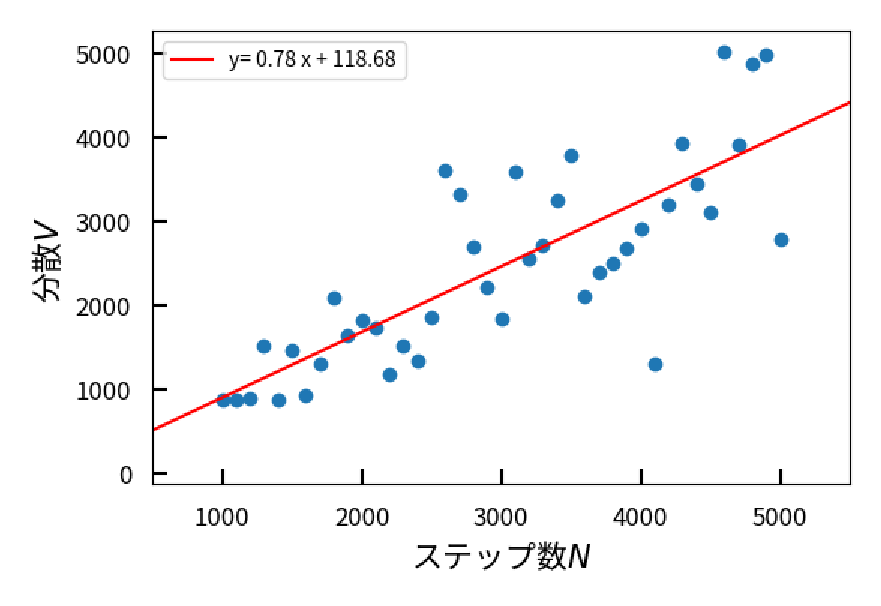
\includegraphics[scale=0.6]{t5.eps}
        \caption{p=0.5,TRIAL=5のときの実行結果}
        \label{t5}
        \end{figure}

        次にTRIAL=30にして実行する.図\ref{t30}にp=0.5,TRIAL=30の条件での実行結果を示す.図\ref{t30}から,
        ステップ数Nと分散Vに強い正の相関があることが読み取れる.さらに,回帰直線がおおよそ$V=N$であることが読み取れる.

        \begin{figure}[H]
            \centering
            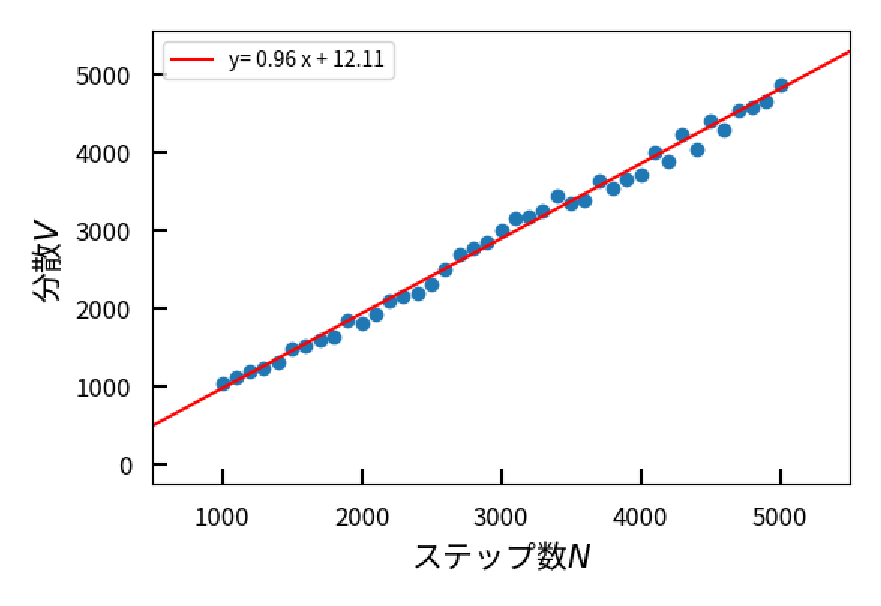
\includegraphics[scale=0.6]{t30.eps}
            \caption{p=0.5,TRIAL=30のときの実行結果}
            \label{t30}
            \end{figure}       

        最後にp=0.7,TRIAL=30の条件で実行する.図\ref{p07}にp=0.7,TRIAL=30の条件での実行結果を示す.図\ref{p07}から,
        単回帰係数が$0.83$と,p=0.5と比較して傾きが緩やかになっていることが読み取れる.

        \begin{figure}[H]
            \centering
            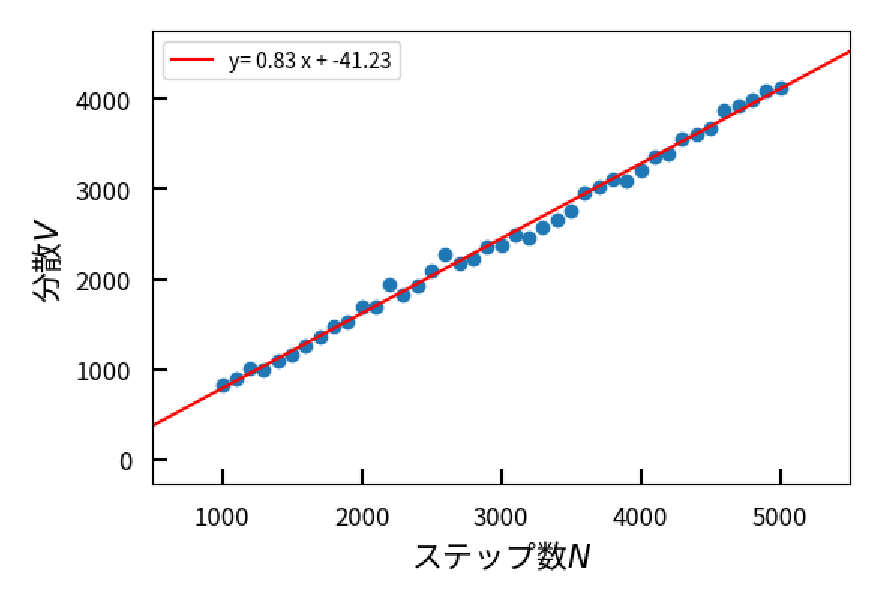
\includegraphics[scale=0.6]{p07.eps}
            \caption{p=0.7,TRIAL=30のときの実行結果}
            \label{p07}
            \end{figure}   

        分散と$N$,$p$の関係について考察する. $S_1,S_2,\dots S_n$,i.i.d(独立同分布)とし,$P(S_i=1)=p,P(S_i=-1)=1-p$とする($L=1$に限定して考える).
        $n \geq 1$に対して確率変数$X_n$を式(\ref{xn})のように定義する.式(\ref{xn})のように定義すると$X_n$は時刻$n$における位置を表している.
        また,この運動がランダムウォークである.

        \begin{eqnarray}
          X_n = S_1 + S_2 + \dots + S_n \label{xn}
        \end{eqnarray}

        $E[X_n]$および$V[X_n]$を計算するために,時刻$n$に位置が$k$である確率$P(X_n = k)$を求める必要がある.確率$P(X_n = k)$を計算するために$W_n$,$L_n$
        という2つの変数を定義する. $S_i=1$なる$i$の個数$W_n$,$S_i=-1$なるiの個数$L_n$とする.このとき,$W_n$は二項分布$Bin(n,p)$に従う. $W_n$,$L_n$を用いると
        $X_n=W_n-L_n$,$n=W_n+L_n$と表せる.これより$X_n+n=2W_n$と表せる.したがって,$X_n=k$は$W_n=\frac{k+n}{2}$と表せる.
        $k+n$が奇数のとき,$\frac{k+n}{2}$は整数にならない.このため,$_n C _\frac{k+n}{2}$は計算できないから,$P(X_n =k)=0$となる.$k+n$が偶数のときは
        $P(X_n=k)$は式(\ref{px})になる.
        \begin{eqnarray}
            P(X_n=k) = P\left( W_n = \frac{n+k}{2} \right) = {}_n C _{\frac{n+k}{2}} p^{\frac{n+k}{2}} (1-p)^{\frac{n-k}{2}} \label{px}
          \end{eqnarray}

          式(\ref{px})は二項分布だから期待値と分散は簡単に計算できる. $X_n$の期待値および分散は式(\ref{ex})および式(\ref{vx})になる.
          \begin{eqnarray}
            E[X_n] &=& E[2W_n -n] = 2np-n = n(2p-1) \label{ex} \\
            V[X_n] &=& V[2W_n -n] = 4V[W_n] = 4np(1-p) \label{vx}
          \end{eqnarray}

          $p=0.5$のとき,期待値と分散を計算してみる.式(\ref{ex})および式(\ref{vx})に$p=0.5$を代入すると式(\ref{ex05})および式(\ref{vx05})のようになる.
          式(\ref{vx05})は,数値計算で求めた分散$V[\Delta x^2(N)]=N$になることを示している.図\ref{t30}で示した回帰係数がおおよそ1になっていること
          から,$p=0.5$のときの分散$V[\Delta x^2(N)]=N$という理論と一致していることがわかる.
          \begin{eqnarray}
            E[X_n] &=&  n(2p-1) = 0 \label{ex05} \\
            V[X_n] &=& 4np(1-p) = n \label{vx05}
          \end{eqnarray}
        
          $p=0.7$のとき,期待値と分散を計算してみる.式(\ref{ex})および式(\ref{vx})に$p=0.7$を代入すると式(\ref{ex07})および式(\ref{vx07})のようになる.
          式(\ref{vx07})は,数値計算で求めた分散$V[\Delta x^2(N)]=0.84N$になることを示している.図\ref{p07}で示した回帰係数がおおよそ0.83になっていること
          から,$p=0.7$のときの分散$V[\Delta x^2(N)]=0.84N$という理論と一致していることがわかる.
          \begin{eqnarray}
            E[X_n] &=&  n(2p-1) = 0.4n \label{ex07} \\
            V[X_n] &=& 4np(1-p) = 0.84n \label{vx07}
          \end{eqnarray}
         
          \section{課題14-2}
          本章では,課題14-2のプログラムおよび実行結果と考察について述べる.
          \subsection{プログラム}
          リスト\ref{kadai142}に課題14-2のコードを示す.リスト\ref{kadai142}のコードはNステップの2次元ランダムウォークを
          1回行うコードであり,複数回呼び出すためにマクロを組んでいる.
          \begin{lstlisting}[basicstyle=\ttfamily\footnotesize, frame=single,label=kadai142,caption=課題14-2のコード]
#include<stdio.h>
#include <stdlib.h>
#include <time.h>
#include <math.h>

// 試行回数n
// 移動距離 L
void randomWalk2(int n,int L){
    double X=0;
    double Y=0;
    double rnd;
    int i;
    printf("%d,%lf,%lf\n",0,0.0,0.0);
    for(i=0;i<n;i++){
        // make random[0,1]
        rnd = (double)rand()/RAND_MAX;
        // make random[0,2pi]
        rnd*=2*M_PI;
        X+=L*cos(rnd);
        Y+=L*sin(rnd);
        printf("%d,%lf,%lf\n",i+1,X,Y);
    }
}

int main(void){
    srand((unsigned) time(NULL));
    randomWalk2(5000,1);
    return 0;
}
          \end{lstlisting}

          \subsection{実行結果と考察}
          リスト\ref{kadai142}のコードをステップ数が100,1000,5000のときについて,それぞれ200回実行した.図\ref{r100}~図\ref{r5000}
          に実行結果を示す.図\ref{r100}はステップ数が100,図\ref{r1000}は1000,図\ref{r5000}は5000のときのグラフである.
          図\ref{r100}~図\ref{r5000}から,ステップ数を大きくすると移動距離の半径が多くなる傾向が読み取れる.

          \begin{figure}[H]
            \centering
            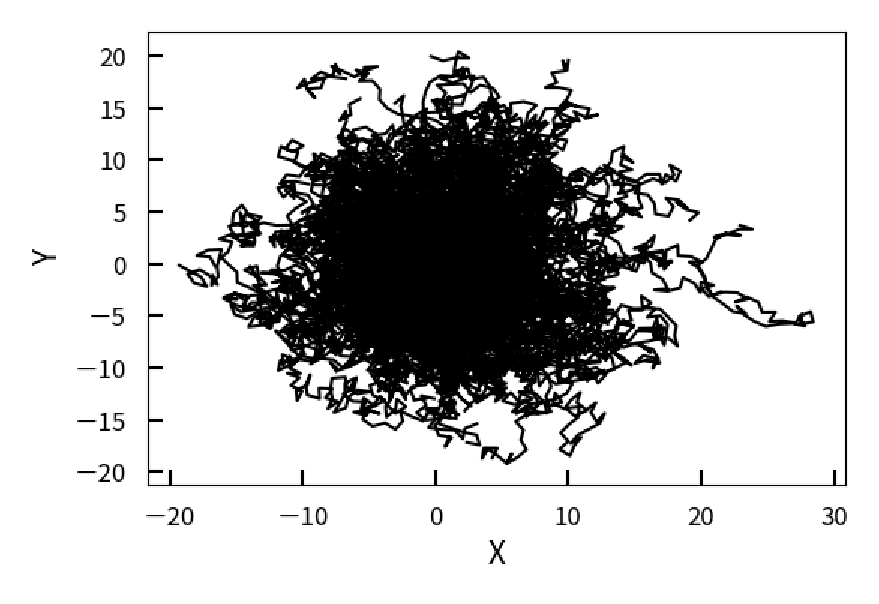
\includegraphics[scale=0.6]{r2-100.eps}
            \caption{ステップ数が100のときの実行結果}
            \label{r100}
            \end{figure}   
        
            \begin{figure}[H]
                \centering
                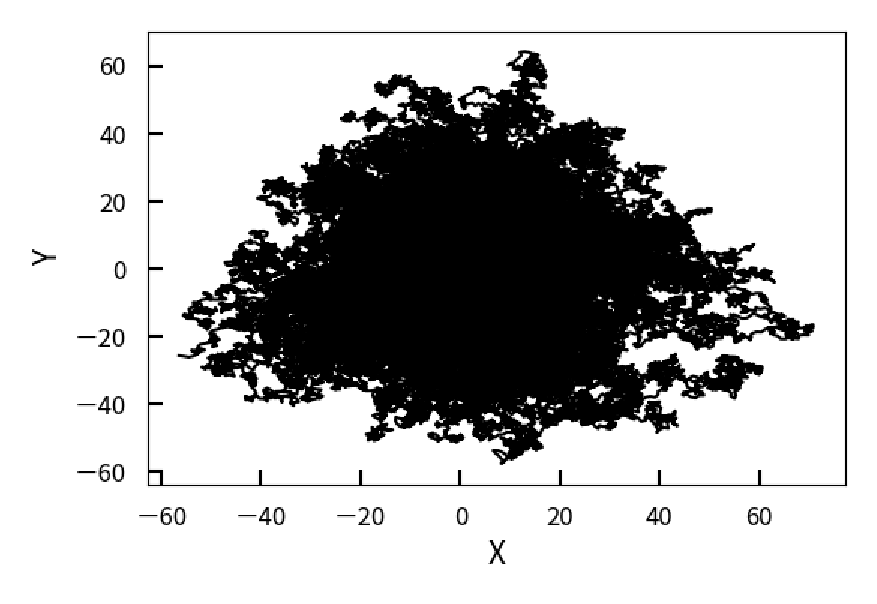
\includegraphics[scale=0.6]{r2-1000.eps}
                \caption{ステップ数が1000のときの実行結果}
                \label{r1000}
                \end{figure}   
        
            \begin{figure}[H]
            \centering
            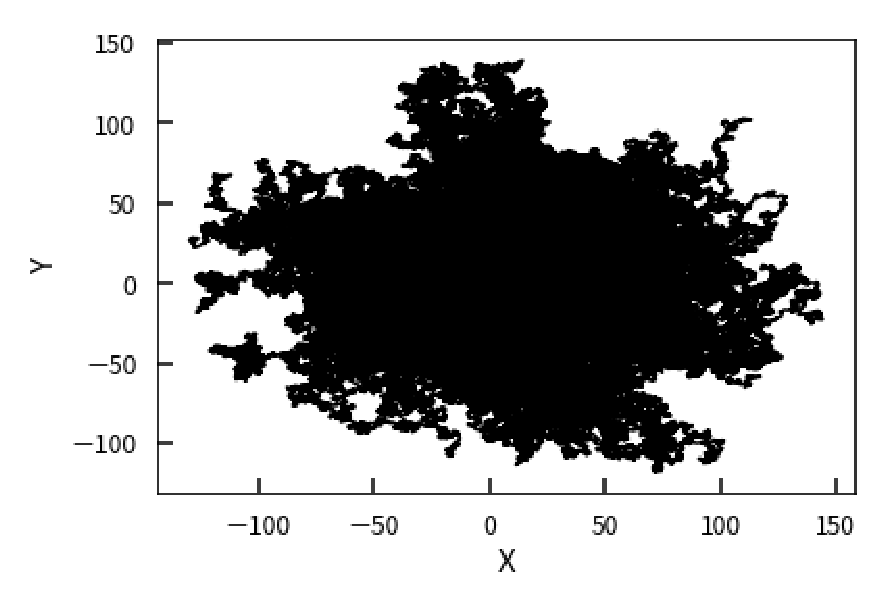
\includegraphics[scale=0.6]{r2-5000.eps}
            \caption{ステップ数が5000のときの実行結果}
            \label{r5000}
            \end{figure}   
            
            ステップ数を大きくしたときの半径について考察する.表\ref{meanvar}にNステップ経過したときの粒子の原点$(0,0)$
            からの距離の平均および標準偏差を示す.表\ref{meanvar}から,Nステップ数後の原点からの距離はおおよそ平均N,標準偏差N
            であることが読み取れる.このことから,2次元ランダムウォークの場合も分散はNになると考えられる.
            
            \begin{table}[H]
            \caption{Nステップ後の距離の平均と標準偏差}
            \label{meanvar}
            \begin{center}
            \begin{tabular}{c|c|c}\hline
                ステップ数 & 平均 & 標準偏差 \\ \hline \hline
                100 & 103.62 & 101.18 \\
                1000 & 964.67 & 855.02 \\
                5000 & 4653.74 & 4475.67 \\ \hline
            \end{tabular}
            \end{center}
            \end{table}

        \begin{thebibliography}{9}
            \bibitem{wakari}  栗原正仁,"わかりやすい数値計算入門",ムイスリ出版,2018
            \bibitem{kiso}  久保田達也,"現代数理統計学の基礎",共立出版社,2020
          \end{thebibliography}
\end{document}

